\documentclass[12pt]{article}
\usepackage[utf8]{inputenc}

\title{Specyfikacja implementacyjna}
\author{Patryk Zaniewski}
\date{11.11.2018}

\usepackage{natbib}
\usepackage{graphicx}
\usepackage{polski}

\begin{document}

\maketitle

\tableofcontents
\newpage

\section{Wstęp}
Program ma na celu rozwiązanie problemu najkorzystniejszej wymiany walut i/lub wyszukania arbitrażu walutowego. Do napisania programu zostanie wykorzystany język Java w wersji 11 oraz środowisko programistyczne Intellij idea 2018 firmy JetBrains.

\section{Opis wykorzystanych algorytmów}
Program poza standardowymi algorytmami wczytania, walidacji oraz wypisania danych będzie zawierał szereg innych algorytmów. Odpowiedzialne one będą za właściwe przechowywanie kursów walut, wyszukanie najkorzystniejszej ścieżki ich wymiany oraz za wyszukanie arbitrażu.
\newline\newline
Algorytm przechowywania walut będzie bazował na strukturze danych zwaną grafem. Implementacja będzie bazowała na liście list. Każdy z jej elementów będzie parą.


 
\section{Diagram klas}
Na poniższym diagramie \emph{Rysunek 1} zostały zobrazowane zależności między klasami w programie. Każda z klas zostanie szczegółowo opisana w kolejnym punkcie. W diagramie zostały pominięte metody get() i set(), jako nie wpływające znacząco na logikę aplikacji - na diagramie mogłyby przysłonić bardziej istotne elementy.

\begin{figure}[h!]
\centering
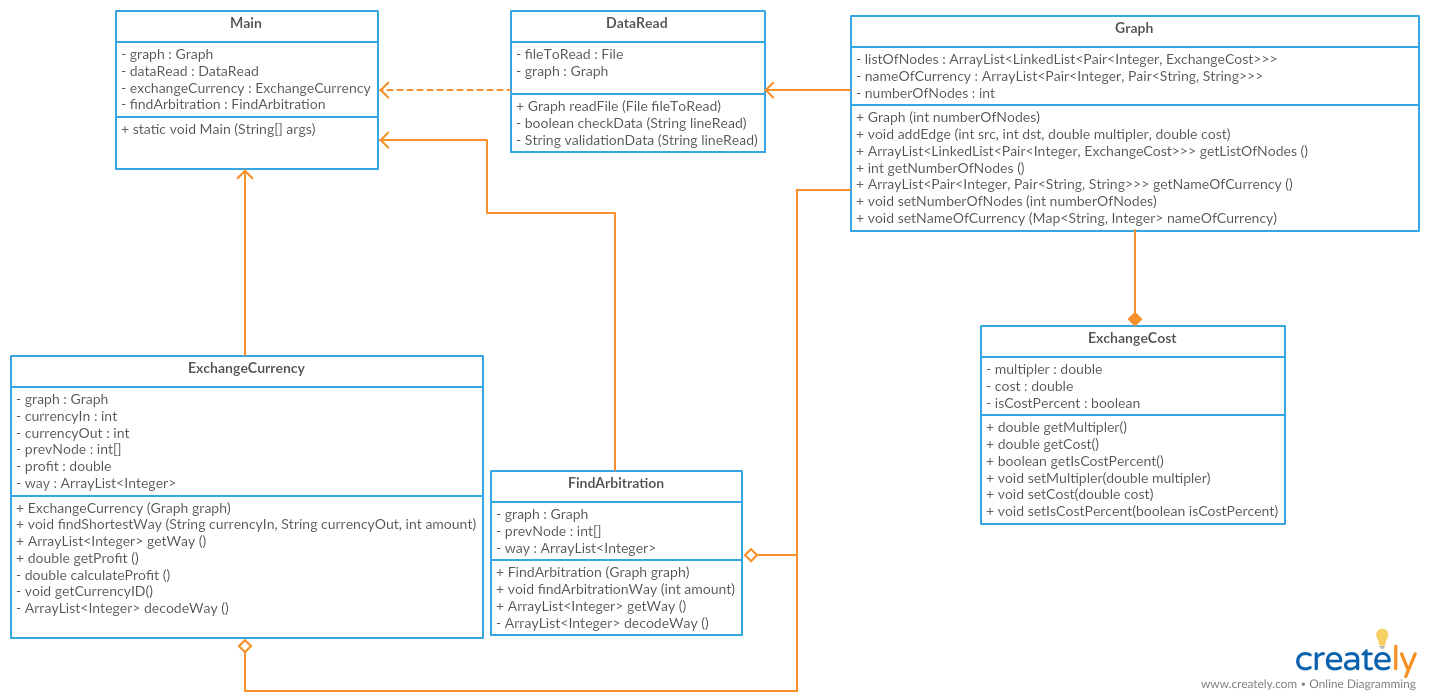
\includegraphics[scale=0.5]{diagram}
\caption{diagram klas}
\label{fig:diagram}
\end{figure}

\section{Opis klas i metod}

\section{Spis zaimportowanych pakietów}
W programie zostaną zaimportowane i użyte pakiety wymienione poniżej. 
\begin{enumerate}
    \item java.lang
    \item java.util
    \item java.io
    
\end{enumerate}

\section{Testy jednostkowe}
Testy jednostkowe generowane będą za pomocą narzędzia JUnit za pomocą którego otrzymamy możliwość sprawdzenia poszczególnych metod w klasach.
Przykładowe testy:
\end{document}
